\documentclass[11pt,e-only]{amsart}
\usepackage[utf8]{inputenc}
\usepackage[english]{babel}

\usepackage{amsmath, amsfonts, amssymb, amsthm}
\usepackage{mathtools}
\usepackage{graphicx}
\usepackage{xcolor}
\usepackage{makecell}
\usepackage{stackengine}
\usepackage{longtable}
\setlength{\tabcolsep}{7pt}
\renewcommand{\arraystretch}{1.2}
\usepackage{comment}
\usepackage{aliascnt}

\usepackage{booktabs}

\usepackage{tikz}
\usetikzlibrary{braids,decorations.pathreplacing}
\usetikzlibrary{matrix,arrows.meta}

\usepackage{multirow}
\usepackage{array}
\usepackage[breaklinks=true]{hyperref}
\usepackage{xurl}
\hypersetup{
    colorlinks,
    linkcolor={blue!80!black},
    citecolor={blue!50!black},
    urlcolor={blue!80!black}
}

\usepackage[capitalize]{cleveref}
\usepackage[margin=3cm]{geometry}

\usepackage{caption}
\usepackage{setspace}
\usepackage{fancyhdr}
\usepackage{subcaption}
\usepackage[normalem]{ulem}
\usepackage[isbn=false,giveninits=true,date=year]{biblatex}
\usepackage{csquotes}


%make biblatex print shortjournal
\renewbibmacro*{journal}{%
  \iffieldundef{shortjournal}
    {%
      \iffieldundef{journaltitle}
        {}
        {%
          \printtext[journaltitle]
            {%
              \printfield[titlecase]{journaltitle}%
              \setunit{\subtitlepunct}%
              \printfield[titlecase]{journalsubtitle}%
             }%
         }%
    }
    {\printtext[journaltitle]{\printfield[titlecase]{shortjournal}}}%
}


% remove url if doi or eprint available
\AtEveryBibitem{%
  \iffieldundef{doi}{}{\clearfield{url}}%
}
\AtEveryBibitem{%
  \iffieldundef{eprint}{}{\clearfield{url}\clearfield{urldate}}%
}

\usepackage{mymacros}

\addbibresource{refs.bib}

\stackMath


%%%%%%%%%%%%%%%%%%%%%%%%%%%%%%%%%%%%%%%%%%%%%%%%%%%%%%%%%%%%%%%%%%%%%%%%%%%%%%%%%%%%%%%%

\title{Links project}

\author[D. Passaro]{Davide Passaro}

\author[L. San Mart\'in Su\'arez]{Lara San Mart\'in Su\'arez}

\thanks{California Institute of Technology, Pasadena, CA 91125, USA}

\date{\today}

\begin{document}

\maketitle

\section{Conventions} False theta $h_n(q)$. Theta function $\psi_n(q)$. We use $\factoreq$ for equality up to a factor $\pm q^j$ for some $j$. We use $\expeq$ whenever we identify a truncated series with a closed formula, and we specify in the main text until what order it holds. All knot and link's orientations follow the KnotInfo convention \cite{knotinfo}.


% In https://arxiv.org/pdf/1106.3948 Def 3.1 they do the opposite notation

\section{Contents}

\begin{enumerate}
    \item Structure of $F_L$ in terms of $\Delta_L$
    \item Pairs $(L_1,L_2)$ and reverse-engineering of $+1/r$ partial surgery
    \item New $F_K$'s of non-fibered knots using partial surgeries
    \item Perturbative expansions of $F_L$'s (do a figure)
    \begin{enumerate}
        \item Positive braid knots
        \item Whitehead
    \end{enumerate}
    \item Surgeries on torus links
    \item $F_L$ vs. ADO? Does $F_L$ read the Hopf invariant/fibered surface? Slopes?
\end{enumerate}

Questions we try to answer: can we use (link, surgery formula) to get new knots? Can we use (link, knots) to get surgery formula?

\section{Preliminaries}

\subsection{Multivariable Alexander polynomial}

\begin{itemize}
    \item Definition, single variable option, Alexander-Conway
    \item Properties
    \item Expansion of its inverse
    \item ``Random walk'' interpretation? (with example)
    \item Proof: homogeneous braid links (it does not vanish + it does have a constant term)
\end{itemize}

% \subsubsection{Definition and properties}

\subsubsection{Definition and properties}



\subsubsection{Computation}

\begin{enumerate}
    \item Applying Fox derivatives to Writinger presentation on a braid
\end{enumerate}

[About our convention of assigning labels to $x$-variables by order of appearance in the braid]

Given a braid $\bd$, consider the tangle obtained by identifying every strand but the left-most one. We call this a partial closure of $\bd$. Enumerate each of the segments in the resulting diagram. Denote $\phi$ the function that sends every segment to the index of the component it belongs to. We construct a square matrix $A^{\bd}=A^{\bd}(x_1,\dots,x_n)\in M_{2n+1}(\Z[x_1,\dots,x_n])$ of size \alert{$2n+1$}, where $n$ is the number of components of the total closure of $\bd$, in the following way: at each crossing, denote by $i$ and $j$ the labels of the incoming overstrand and understrand, and by $i^+$ and $j^+$ the labels of the outgoing overstrand and understrand, respectively. Let $s\in\{\pm1\}$ denote the sign of the crossing. Then, the values of $A^{\bd}$ in the $i$ and $j$ columns are given by the following rules:
\begin{equation}\label{eq:A-rules}
\begin{split}
    &A_{i,i^+}^\bd=\begin{cases}
        x_{\phi(j)} &\quad \text{if } s=+1 \\
        \frac{1}{x_{\phi(j)}} &\quad \text{if } s=-1 \\
    \end{cases}
    \, , \hspace{1em}
    A_{i,j^+}^\bd=\begin{cases}
        1-x_{\phi(i)} &\quad \text{if } s=+1 \\
        \frac{x_{\phi(i)}}{x_{\phi(j)}}\left(1-\frac{1}{x_{\phi(i)}}\right) &\quad \text{if } s=-1 \\
    \end{cases}
    \, , \hspace{1em}
    A_{j,i^+}^\bd=0
    \, , \\&
    A_{j,j^+}^\bd=1
    \, , \hspace{1em}\text{and}\hspace{1em}
    A_{i,k}=A_{j,k}=0 \quad \text{if } k\neq i^+,j^+.
    \end{split}
\end{equation}

The reader should note that this is the result of applying the free Fox derivatives calculus to the Writinger presentation of a link complement represented by a braid [...].

Then,
\begin{equation}
    \Delta_{\mathrm{cl}(\bd)}(x_1,\dots,x_n) = \left(\prod_{i=1}^n x_i^{-\frac{1}{2}\left(-N_i+\sum_{j=1}^n lk(i,j)\right)}\right) \frac{\det{\left(I_{N}-A^\bd\right)}}{1-x_1},
\end{equation}
\alert{up to overall sign}where $lk(i,j)$ denotes the linking number between the $i$-th and $j$-th component and $n_j$ denotes the number of strands of the $j$-th component. For simplicity later, we define $M^\bd:=I_{N}-A^\bd$. % We can change it to be the rot number too

\begin{remark}
    If you close the braid, you can do the same by substituting $A$ by $\hat{A}_j^\bd=\hat{A}^\bd_j(x_1,\dots,x_n)$, the resulting matrix from deleting the $j$-th row and column from $A^\bd(x_1,\dots,x_n)$, where $A$ is obtained after doing the total trace. Then,
\begin{equation}
    \Delta_{\mathrm{cl}(\bd)}(x_1,\dots,x_n) \simeq \frac{\det{\left(I_{N}-\hat{A}^\bd_j\right)}}{1-x_{\phi(a_j)}}
\end{equation}
for any $1 \leq j\leq N$. This is secretly what we are doing by keeping one strand open. The result is independent on what $j$ we choose. The relation with our way of doing it is equivalent of choosing $j=1$.
\end{remark}

\begin{example} ($H^\pm$) Let $H^{\pm}$ denote the positive and negative Hopf links, with braid words $\sigma_1^2$ and $\sigma_1^{-2}$ respectively. Labeling the braid segments as in Figure [...], we construct the matrices
\begin{equation}
    A^{H^+}=\begin{pmatrix}
    0 & x_2 & 0 & 0 & 1-x_1 \\
    0 & 0 & 1 & 0 & 0\\
    0 & 0 & 0 & 0 & 0 \\
    0 & 0 & 0 & 0 & 1 \\
    0 & 0 & 1-x_2 & x_1 & 0 \\
    \end{pmatrix},
    \hspace{1em}
    A^{H^-}=\begin{pmatrix}
    0 & 1 & 0 & 0 & 0 \\
    0 & 0 & \frac{1}{x_2} & \frac{x_1}{x_2}\left(1-\frac{1}{x_1}\right) & 0 \\
    0 & 0 & 0 & 0 & 0 \\
    0 & \frac{x_2}{x_1}\left(1-\frac{1}{x_2}\right) & 0 & 0 & \frac{1}{x_1} \\
    0 & 0 & 0 & 1 & 0 \\
    \end{pmatrix}
\end{equation}
and
\begin{equation}
    \frac{\det\left(I_5-A^{H^+}\right)}{1-x_1}=\frac{1-x_1}{1-x_1}=1, \hspace{2em}\frac{\det\left(I_5-A^{H^-}\right)}{1-x_1}=\frac{x_1^{-1}(1-x_1)}{1-x_1}\factoreq 1.
\end{equation}
\end{example}
% PREFACTORS DO NOT WORK IN THIS CASE?

\begin{example} ($T(2,4)^*$) Let $T(2,4)^*$ be the boundary of the twisted annuli with 2 full twists, as depicted in Figure [...]. We call it $T(2,4)^*$ as it agrees with the torus link $T(2,4)$ as unoriented links. However, as oriented links they are different: in particular, $T(2,4)$ is fibered, while $T(2,4)^*$ is not. Consider the braid representative of $T(2,4)^*$ given by $\bd=\sigma_2^2\sigma_1\sigma_2^{-1}\sigma_1$. 

In Figure [...] we assign labels to each of the segments of the braid $\bd$. For simplicity, we will maintain the same label when going through the understrand, since this will not change the end result, but it will make our example more succinct and didactic. We obtain the matrix:
\begin{equation}\label{eq:T24*-matrix}
    A^{\bd} = \begin{pmatrix}
        0 & x_2 & 0 & 0 & 0 & 1-x_1 \\
        0 & 0 & x_2 & 0 & 0 & 1-x_1 \\
        0 & 1-x_1^{-1} & 0 & x_1^{-1} & 0 & 0 \\
        0 & 0 & 0 & 0 & 0 & 0 \\
        0 & 1-x_2 & 0 & 0 & 0 & x_1 \\
        0 & 0 & 0 & 1-x_2 & x_1 &0 \\
    \end{pmatrix}
\end{equation}
and the polynomial
\begin{equation}
\begin{split}
    \Delta_{T(2,4)^*}(x_1,x_2)&=x_1^{-\frac{1}{2}(-2-1+2)}x_2^{-\frac{1}{2}(-1+2)}\frac{\det\left(I_7-A^\bd\right)}{1-x_1} \\&= x_1^{\frac{1}{2}}x_2^{-\frac{1}{2}}\frac{(1-x_1)x_1^{-1}(x_1+x_2)}{1-x_1} = x_1^{-\frac12}x_2^{-\frac12}\left(x_1+x_2\right),      
\end{split}
\end{equation}
which agrees with the Alexander polynomial of $T(2,4)^*$.
\end{example}

\subsubsection{Interpretation as a sum over multicycles}

We can express the multivariable Alexander as
\begin{equation}
    \Delta_{\mathrm{cl}(\bd)}(x_1,\dots,x_n) = \left(\prod_{i=1}^n x_i^{-\frac{1}{2}\left(-N_i+\sum_{j=1}^n lk(i,j)\right)}\right)\frac{1}{1-x_1}\sum_{\sigma\in S_N} \sgn{\sigma} \,M_{1,\sigma(1)}\cdots M_{N,\sigma(N)}
\end{equation}
where we set $\phi(a_1):=x_1$ by convention. The only permutations $\sigma$ that have non-trivial contribution to $\Delta_{\mathrm{cl}(\bd)}(x_1,\dots,x_n)$ satisfy that $\sigma(i)\in\{i,i^+,j^+\}$ if $i$ is the incoming segment of the overstrand of a crossing, $\sigma(j)\in\{j,j^+\}$ if $j$ is the incoming segment of the understrand, and $\sigma(k)=k$ if $k$ is the top segment of the open strand.

[Definition of simple multicycles and their weights]

Therefore, we can write
\begin{equation}
    \Delta_{\mathrm{cl}(\bd)}(x_1,\dots,x_n) = \left(\prod_{i=1}^n x_i^{-\frac{1}{2}\left(-N_i+\sum_{j=1}^n lk(i,j)\right)}\right) \frac{1}{1-x_1} \sum_{c\in C} (-1)^{|c|} W(c).
\end{equation}

This model is called the `jump up' model and has been studied in [...].

\begin{example}\label{ex:T24*-cycles} ($T(2,4)^*$) Let $c_1,c_2$ and $c_3$ be the cycles in Figure [...]. Then, the set of simple multicycles that do not go through the open strand are $C=\{\emptyset,c_1,c_2,c_1+c_2,c_3\}$, and
\begin{equation*}
\begin{split}
    \sum_{c\in C} (-1)^{|c|}W(c)&=1+(-1)^{|c_1|}W(c_1)+(-1)^{|c_2|}W(c_2)+(-1)^{|c_1|+|c_2|}W(c_1)W(c_2)+(-1)^{|c_3|}W(c_3)
    \\&=1-x_1^2-x_2(1-x_1^{-1})+x_1^2x_2(1-x_1^{-1})-x_1(1-x_1)(1-x_2)\\&=(1-x_1)x_1^{-1}(x_1+x_2),
\end{split}
\end{equation*}
which agrees with the determinant computed from \cref{eq:T24*-matrix}.
\end{example}

% Jump-down model:
\begin{comment}

\begin{remark} There is a dual model to the ``jump-up'' model called the ``jump-down'' model of the multivariable Alexander polynomial. In that, we change the convention of understrand and overstrand, given that $\Delta_{m(L)}(x_1,\dots,x_n)=?$. 
\end{remark}
    
\end{comment}

\subsection{The inverse of the Alexander polynomial}

% Alert: clarify conventions
We are interested in the inverse of the multivariable Alexander polynomial when we consider the variables $x_1,\dots,x_n$ near $0$. When we are dealing with a knot $K$, the Alexander polynomial satisfies the crucial property of \alert{$\Delta^+_K(0)\neq 0$}, which makes $\Delta_K$ a unit in the ring $\Q[[x]]$. However, in the case of a link $L$ with more than one component, $\Delta_L(0,\dots,0)$ may be zero. We distinguish two cases, depending on whether $\Delta_L$ is a unit in the ring $\Q[[x_1,\dots,x_n]]$ or not. 

In the first case, there is a (unique) inverse of $\Delta_L$ in the ring $\Q[[x_1,\dots,x_n]]$. Take as an example the link $T(2,4)$, computed as the closure of the braid word $\sigma_1^4$. Up to multiplication by monomials in $x_1,x_2$, its multivariable Alexander polynomial is $1+x_1x_2$, and its inverse in the ring $\Z[[x_1,x_2]]\subset \Q[[x_1,x_2]]$ is the power series $\sum_{n\geq 0}(-1)^n x_1^n x_2^n$.

In the second, in order to define an inverse of $\Delta_L$ when it has a zero at the origin, we need to expand the ring in which we are working. With the same goal in mind, [...] introduced the \textit{field of iterated Laurent series}, \[\Q\langle\langle x_1,x_2,\dots,x_n\rangle\rangle:=\Q((x_1))((x_2))\cdots((x_n)),\] which can be defined iteratively as follows: $\Q\langle\langle x_1,x_2,\dots,x_n\rangle\rangle$ is the field of Laurent power series in $x_n$ with coefficients in $\Q\langle\langle x_1,\dots,x_{n-1}\rangle\rangle$, where $\Q\langle\langle x\rangle\rangle:=\Q((x))$ is the field of formal Laurent power series in $x$. In short, we will write $\Q\langle\langle \textbf{x}\rangle\rangle$.
% https://arxiv.org/pdf/math/0405133, Chapter 2

% [...], the case of multivariable polynomials is more subtle. While one would like for the expansion of the inverse Alexander polynomial to be an element of the ring $\Q[[\mathbf{x}]]$, in analogy to the case of knots, this is not always the case. 

The field $\Q\langle\langle \textbf{x}\rangle\rangle$ has a fundamental structure defined as follows: consider the reverse lexicographic ordering in $\Z^n$, for which $(m_1,\dots,m_n)\leq (r_1,\dots,r_n)$ if and only if there exists an $i$ such that $m_i<r_i$ and $m_j=k_j$ for all $j> i$. Recall that a totally ordered set is well-ordered if every non-empty subset contains a minimal element.  % This induces an ordering $\preceq$ in $\Q[\textbf{x}^{\pm1}]$, where $\mathbf{x}^\mathbf{m} < \mathbf{x}^\mathbf{r}$ if and only if $\mathbf{m}\leq \mathbf{r}$ in the reverse lexicographic ordering. 
Then, the elements of $\Q\langle\langle \textbf{x}\rangle\rangle$ are precisely the Laurent power series with a well-ordered support ([..., Proposition 2.1-2]). From this point of view, we can view the field $\Q\langle\langle \textbf{x}\rangle\rangle$ as the Laurent power series in $\Q$ with support in $\mathbf{x}$ defined in $1>>x_1>>x_2>>\dots>>x_n$, where $x_i$ are complex variables. % \alert{see refs}
% Define support and well-define, the notation \mathbf{x}^\mathbf{n} etc. in a notation section

Let $f\in\Z[\mathbf{x}]$. Since $\Z[\mathbf{x}]$ can be embedded into $\Q\langle\langle\mathbf{x}\rangle\rangle$, there exists an element of its support $\mathbf{k}$ that is minimal under the reverse lexicographic ordering. We call $c\mathbf{x}^\mathbf{k}$ the initial term of $f$, where $c$ is the coefficient of $\mathbf{x}^\mathbf{k}$ in $f$. Then, $\frac{1}{c}\mathbf{x}^{-\mathbf{k}}f$ is a unit in $\Q\langle\langle\mathbf{x}\rangle\rangle$ with constant term $1$, and we can define its inverse in $\Q\langle\langle\mathbf{x}\rangle\rangle$, which will have $1$ as initial term as well. For more details, see [..., Lemma 2.1-6].

Obviously, this is true for every permutation of the $x_i$ variables. Given $\sigma\in S_{n}$, there exists a $\mathbf{k}_\sigma$ in the support of $f$, minimal under the reverse lexicographic ordering, and a $c_{\sigma}\in\Z$, such that $\frac{1}{c_\sigma}\mathbf{x}^{-\mathbf{k}_\sigma}f$ is a unit of $\Q\langle\langle \mathbf{x}_\sigma\rangle\rangle=\Q\langle\langle x_{\sigma(1)},\dots,x_{\sigma(n)}\rangle\rangle$ with constant term $1$. Therefore, given a polynomial $f\in\Z[\mathbf{x}]$, we can consider its inverse in the fields $\{\Q\langle\langle \mathbf{x}_\sigma\rangle\rangle\}_{\sigma\in S_n}$, which gives $n!$ potential candidates for the power series expansion of ``$\frac{1}{f}$''.

\begin{example} Consider $f(x_1,x_2)=x_1+x_2$. If we view $f$ as an element of $\Q\langle\langle x_1,x_2\rangle\rangle$, under the embedding of $\Z[x_1,x_2]$ into $\Q\langle\langle x_1,x_2\rangle\rangle$, the initial term of $f$ is $x_1$, and the inverse of $f$ is
\begin{equation}
    \frac{1}{x_1\left(1+\frac{x_2}{x_1}\right)} = \frac{1}{x_1}\sum_{n\geq 0} (-1)^n\left(\frac{x_2}{x_1}\right)^n.
\end{equation}
On the other hand, if we view $f$ as an element of $\Q\langle\langle x_2,x_1\rangle\rangle$, its initial term is $x_2$, and its inverse is the iterated Laurent series
\begin{equation}
    \frac{1}{x_2\left(1+\frac{x_1}{x_2}\right)} = \frac{1}{x_2}\sum_{n\geq 0} (-1)^n\left(\frac{x_1}{x_2}\right)^n.
\end{equation}
\end{example}

\begin{comment}

\begin{example} Consider $f(x_1,x_2,x_3)=x_1x_2^2+x_2^2x_3+x_1x_2x_3^2$. Then, the expansion of $\frac{1}{f}$ in the fields $\Q\langle\langle x_1,x_2,x_3\rangle\rangle$ and $\Q\langle\langle x_2,x_1,x_3\rangle\rangle$ is given by
\begin{equation}
    \frac{1}{f} = \frac{1}{x_1x_2^2}\frac{1}{\left(1+\frac{x_3}{x_1}+\frac{x_3^2}{x_2}\right)} = \frac{1}{x_1x_2^2} \sum_{n\geq 0}(-1)^n\left(\frac{x_3}{x_1}+\frac{x_3^2}{x_2}\right)^n,
\end{equation}
in the fields $\Q\langle\langle x_1,x_3,x_2\rangle\rangle$ and $\Q\langle\langle x_3,x_1,x_2\rangle\rangle$ by
\begin{equation}
    \frac{1}{f} = \frac{1}{x_1x_2x_3^2}\frac{1}{\left(1+\frac{x_2}{x_3^2}+\frac{x_2}{x_1x_3}\right)} = \frac{1}{x_1x_2x_3^2} \sum_{n\geq 0}(-1)^n\left(\frac{x_2}{x_3^2}+\frac{x_2}{x_1x_3}\right)^n,
\end{equation}
and in the fields and $\Q\langle\langle x_2,x_3,x_1\rangle\rangle$ and $\Q\langle\langle x_3,x_2,x_1\rangle\rangle$ by
\begin{equation}
    \frac{1}{f} = \frac{1}{x_2^2x_3}\frac{1}{\left(1+\frac{x_1}{x_3}+\frac{x_1x_3}{x_2}\right)} =  \frac{1}{x_2^2x_3} \sum_{n\geq 0}(-1)^n\left(\frac{x_1}{x_3}+\frac{x_1x_3}{x_2}\right)^n.
\end{equation}
\end{example}

\end{comment}

\begin{table}[]
    \centering
    \begin{tabular}{c|c|c}
        Field & Initial term of $f$ & Iterated Laurent expansions of $1/f$ \\
        $\Q\langle\langle x_1,x_2,x_3\rangle\rangle$ & $x_1x_2^2$ & $\frac{1}{x_1x_2^2} \sum_{n\geq 0}(-1)^n\left(\frac{x_3}{x_1}+\frac{x_3^2}{x_2}\right)^n$ \\
        $\Q\langle\langle x_1,x_3,x_2\rangle\rangle$ & $x_1x_2x_3^2$ & $\frac{1}{x_1x_2x_3^2} \sum_{n\geq 0}(-1)^n\left(\frac{x_2}{x_3^2}+\frac{x_2}{x_1x_3}\right)^n$ \\
        $\Q\langle\langle x_2,x_1,x_3\rangle\rangle$ & $x_1x_2^2$ & $\frac{1}{x_1x_2^2} \sum_{n\geq 0}(-1)^n\left(\frac{x_3}{x_1}+\frac{x_3^2}{x_2}\right)^n$ \\
        $\Q\langle\langle x_2,x_3,x_1\rangle\rangle$ & $x_2^2x_3$ & $\frac{1}{x_2^2x_3} \sum_{n\geq 0}(-1)^n\left(\frac{x_1}{x_3}+\frac{x_1x_3}{x_2}\right)^n$ \\
        $\Q\langle\langle x_3,x_1,x_2\rangle\rangle$ & $x_1x_2x_3^2$ & $\frac{1}{x_1x_2x_3^2} \sum_{n\geq 0}(-1)^n\left(\frac{x_2}{x_3^2}+\frac{x_2}{x_1x_3}\right)^n$ \\
        $\Q\langle\langle x_3,x_2,x_1\rangle\rangle$ & $x_2^2x_3$ & $\frac{1}{x_2^2x_3} \sum_{n\geq 0}(-1)^n\left(\frac{x_1}{x_3}+\frac{x_1x_3}{x_2}\right)^n$ \\
    \end{tabular}
    \caption{Example for $f(x_1,x_2,x_3)=x_1x_2^2+x_2^2x_3+x_1x_2x_3^2$.}
    \label{tab:ex:inverse-3-vars}
\end{table}

\begin{comment}
    
\begin{table}[]
    \centering
    \begin{tabular}{c|c}
        Field & Inverse of $f$ \\ % Change because we would have to kill that prefactor ish
        $\Q_{\langle x_1x_2^2\rangle}[[x_1,x_2,x_3]]$ & $\frac{1}{x_1x_2^2} \sum_{n\geq 0}(-1)^n\left(\frac{x_3}{x_1}+\frac{x_3^2}{x_2}\right)^n$ \\
        $\Q_{\langle x_1x_2x_3^2\rangle}[[x_1,x_3,x_2]]$ & $\frac{1}{x_1x_2x_3^2} \sum_{n\geq 0}(-1)^n\left(\frac{x_2}{x_3^2}+\frac{x_2}{x_1x_3}\right)^n$ \\
        $\Q_{\langle x_2^2x_3\rangle} [[x_2,x_3,x_1]]$ & $\frac{1}{x_2^2x_3} \sum_{n\geq 0}(-1)^n\left(\frac{x_1}{x_3}+\frac{x_1x_3}{x_2}\right)^n$ \\
    \end{tabular}
    \caption{Example for $f(x_1,x_2,x_3)=x_1x_2^2+x_2^2x_3+x_1x_2x_3^2$.}
    \label{tab:ex:inverse-3-vars-cones}
\end{table}

\end{comment}

In our case, we are interested in the number of different ``$\frac{1}{f}$'' series we can obtain, depending on the support of $f$. Often times, the expressions of $\frac{1}{f}$ defined in the different fields of iterated Laurent series will coincide, as in the example in \cref{tab:ex:inverse-3-vars}. To answer how many different inverses of $f$ we can define, we would like for the $\frac{1}{f}$ with the same expression to be defined in the same ring. In order to do this, we can use the theory developed in [...]. In spirit, the objective is the same as before: we want to extend the ring we work in, so we can define inverse of polynomials in multiple variables; but now the ring we consider will be defined using the support of $f$.

First, we must introduce the notion of a \textit{cone}. Let $C$ be a rational, finitely-generated, line-free, $n$-dimensional cone; i.e. a subset of $\R^n$ such that there exist $s\in\N$ and $\mathbf{v}_1,\cdots,\mathbf{v}_s\in\Z^n$ with $C=\{z_1\mathbf{v}_1+\cdots+z_s\mathbf{v}_s \mid z_1,\dots,z_n \geq 0 \}$ and $-\mathbf{v}_i\notin C$ for all $i$. Define the ring \[\Q_C[[\mathbf{x}]]:=\{f(\mathbf{x}) \mid \textrm{supp}\;f(\mathbf{x})\subseteq C\}\] (see [...] for more details on its ring structure). By [..., ...], the ring of units of $\Q_C[[\mathbf{x}]]$ is equal to the functions $f(\mathbf{x})=\sum_{\mathbf{k}\in C} a_\mathbf{k}\mathbf{x}^\mathbf{k}$ with $a_\mathbf{0}\neq 0$.

Now let $\{c_{\mathbf{i}_1}\mathbf{x}^{\mathbf{i}_1},\dots,c_{\mathbf{i}_m}\mathbf{x}^{\mathbf{i}_m}\}$ be the set of distinct initial terms of $f$ under the embedding of $\Z[[\mathbf{x}]]$ into the $n!$ fields of iterated Laurent series, with $0\leq m\leq n$. Then, $h_k:=\frac{1}{c_{\mathbf{i}_k}}\mathbf{x}^{-\mathbf{i}_k}f$ is a unit of the ring $\Q_{C_{\mathbf{i}_k}}[[\mathbf{x}]]$, where $C_{\mathbf{i}_k}$ is finitely generated by the set $\{\mathbf{v}\mid \mathbf{v}\neq \mathbf{i}_k \text{ and } \mathbf{v}+\mathbf{i}_k\in\textrm{supp}\;f\}\bigcup \{\mathbf{i}_\mathbf{k}\}$. We can identify $\frac{1}{c_{\mathbf{i}_1}}\mathbf{x}^{-\mathbf{i}_1}\frac{1}{h_1}\in\Q_{C_{\mathbf{i}_1}}[[\mathbf{x}]],\cdots,\frac{1}{c_{\mathbf{i}_m}}\mathbf{x}^{-\mathbf{i}_m}\frac{1}{h_m}\in\Q_{C_{\mathbf{i}_m}}[[\mathbf{x}]]$ as being the $m$ inverses of $f$, defined in suitable rings.

\begin{example} Let $f(x_1,x_2,x_3)=x_1x_2^2+x_2^2x_3+x_1x_2x_3^2$. From \cref{tab:ex:inverse-3-vars} we can see that the set of distinct initial terms of $f$ is $\{\mathbf{x}^{(1,2,0)},\mathbf{x}^{(0,2,1)},\mathbf{x}^{(1,1,2)}\}$. We define the three cones
\begin{equation}
\begin{split}
    C_{(1,2,0)}&:=\{z_1(1,2,0)+z_2(-1,0,1)+z_3(0,-1,2)\mid z_1,z_2,z_3\geq 0\}, \\
    C_{(0,2,1)}&:=\{z_1(0,2,1)+z_2(1,0,-1)+z_3(1,-1,1)\mid z_1,z_2,z_3\geq 0\}, \\
    C_{(1,2,0)}&:=\{z_1(1,1,2)+z_2(0,1,-2)+z_3(-1,1,-1)\mid z_1,z_2,z_3\geq 0\}.
\end{split} 
\end{equation}
Let us take the cone $C_{(1,2,0)}$ as an example. The Laurent polynomial $h_{(1,2,0)}(x_1,x_2,x_3):=\frac{1}{x_1x_2^2}f(x_1,x_2,x_3)=1+\frac{x_3}{x_1}+\frac{x_3^2}{x_2}$ has support in the cone $C_{(1,2,0)}$ and its initial term is $1$. It is invertible in the ring $\Q_{C_{(1,2,0)}}[[x_1,x_2,x_3]]$, with inverse
\begin{equation}
    \sum_{n\geq 0} (-1)^n\left(\frac{x_3}{x_1}+\frac{x_3^2}{x_2}\right)^n
\end{equation}
which is clearly an element of $\Q_{C_{(1,2,0)}}[[x_1,x_2,x_3]]$. It is therefore natural to consider the inverse of $f$ to be $\frac{1}{x_1x_2^2}\sum_{n\geq 0} (-1)^n\left(\frac{x_3}{x_1}+\frac{x_3^2}{x_2}\right)^n$, which agrees with the result obtained from one of the iterated Laurent expansion of $1/f$.
% \alert{finish with the multiplication final and check still element of}
\end{example}

% This will be given by the number of distinct initial terms of $f$ as an element of $\Q\langle\langle \mathbf{x}_\sigma\rangle\rangle$ for $\sigma\in S_n$. For example, in \cref{tab:ex:inverse-3-vars}, each of the monomials in $f(x_1,x_2,x_3)=x_1x_2^2+x_2^2x_3+x_1x_2x_3^2$ appear as the initial term of $f$ for two permutations, which gives $3!-1!-1!-1!=6-3=3$ total different expansions of $f$. \alert{This does not make sense because they are defined in different rings!}

% permutations $\sigma\in S_n$ with distinct minimal elements in the support of $f$ in the reverse lexicographic ordering induced by $\sigma$, where we are using implicitly the embedding of $\Z[\mathbf{x}]$ into $\Q\langle\langle \mathbf{x}_\sigma\rangle\rangle$. From this point of view, it might be more natural to consider the fields defined in [...].

% Alternatively, one can express the problem as follows: [the cones approach, where each cone $C_j$ will correspond to one or more of the regions above.]

% https://www.sciencedirect.com/science/article/pii/S0723086913000054?via%3Dihub


% Decide if we want to include formally like this or not:
\begin{comment}

\begin{proposition}[Meta-proposition] Let $f(\mathbf{x})\in\Z[\mathbf{x}]$ such that $f(\mathbf{0})=0$. Then, the number of minimal cones $C_j$ (minimal w.r.t inclusion) such that there exist $\mathbf{e}_j$ and $c\in\Z$ with $\frac{1}{c}\mathbf{x}^{-\mathbf{e}_j}f(\mathbf{x})\in\Q_{C_j}[[\mathbf{x}]]^\times$ is given by the different monomials in $f$ minimal by the lexicographic order \alert{(explain)} % n! - (number of fields it appears in -1)! - (number of fields it appears in -1)! - ... % Check this formula
\end{proposition}

\end{comment}

\begin{proposition} Let $\varphi_\sigma$ be the embedding of $\Z[\mathbf{x}]$ into $\Q\langle\langle \mathbf{x}_\sigma \rangle\rangle$ for $\sigma\in S_n$. Then, there are as many different expansions of $\frac{1}{\Delta_L(\mathbf{x})}$ as the cardinality of the set \[\{c_\sigma \mathbf{x}^\sigma \mid \sigma\in S_n\text{ and } c_\sigma \mathbf{x}^\sigma \text{ is the initial term of }\varphi_\sigma(f)\}.\]
% [Multivariable Alexander has multiple expansions depending on the cones, and there will be at most $s!$ where $s$ is the number of components of the link]
\end{proposition}

\subsubsection{Homogeneous braid links}

% Define \Delta^+
\begin{proposition} Let $\bd$ be a homogeneous braid and $L$ its closure. Then, $\alert{|\Delta^+_L(\mathbf{0})| = 1}$. 
\end{proposition}

% Fix labels of the negative crossings vs. label of the # components
\begin{proof} Denote by $n_-$ the number of negative generators in $\bd$. Let $c_-$ be a multicycle of $n_-$ components, whose $i$-th component starts at the incoming overstrand of the first appearance of $\alert{\sigma_i^{-1}}$ and jumps down to the outgoing understrand at every appearance of $\sigma_i^{-1}$ (see [...]). Given the rules in \cref{eq:A-rules}, the weight of $c_-$ in the determinant computation of $\Delta_L(\mathbf{x})$ is
\begin{equation}
    W(c_-) = \prod_{i=1}^n x_i^{-k_i} (1-x_i)^{s_i}
\end{equation}
for some $k_i,s_i\geq 0$. Moreover, $c_-$ minimizes the exponents of all $x_i$ variables simultaneously, as the weight of any other multicycle $c$ in the braid must have minimal $x_i$ exponent greater of equal than $-k_i$. Therefore, we get that
\begin{equation}
    \alert{\Delta^+_L(\mathbf{x})}=\left(\prod_{i=1}^nx_i^{\frac12\left(-N_j+\sum_{j=1}^n lk(i,j)\right)+k_i}\right)\Delta_L(\mathbf{x}) = 1+p(\mathbf{x}),
\end{equation} % Check on some example
where $p(\mathbf{x})\in\Z[\mathbf{x}]$.
\end{proof}

\begin{corollary} The multivariable Alexander polynomial of a homogeneous braid link is invertible in $\Z[[\mathbf{x}]]$.
\end{corollary}

\subsection{Inverted state sum}

\begin{itemize}
    \item Re-definition for links, given the above; i.e. stress that the inverted state sum involves taking one of the cycles above and inverting. In practice, we need one that reads the minimal power. Perhaps this is good time to introduce my meta-proposition below, or adding a section about cones etc.
    \item Proof that we recover 1/Alexander?
    \item MMR for links
    \item Introduction of single-variable FL
\end{itemize}

In \cite{Park21} \alert{check} it was proven that
\begin{equation}
    F_L(\mathbf{x},1+h)=\prod_{i=1,\cdots,s} \left(x_i^{\frac12}-x_i^{-\frac12}\right) \left(\frac{1}{\Delta_L(\mathbf{x})}+\sum_{j=1}^\infty h^j \frac{P_j^K(\mathbf{x})}{\Delta^{2j+1}_L(\mathbf{x})}\right)
\end{equation}
whenever the r.h.s. is defined.

For nice links, the coefficients of $F_L$ are finite Laurent polynomials in $q$. Therefore, we can evaluate the result at $q=1$ and obtain an $s$-variable series in $\mathbf{x}$, which must agree with the expansion near zero of the inverse multivariable Alexander polynomial. This constrains the structure of the corresponding $F_L$ invariant, and we distinguish three different cases. See \cref{tab:expansion-inverse-wrt-zeros}.

\subsubsection{$R$-matrices}

\begin{remark}
% [Park21]
Notice that our convention differs from the one in [...]. This is partly due to the conjecture 
\begin{equation}\label{eq:ADO-FL} % For links, what is the correct normalization factor missing?
    \lim_{q\rightarrow \zeta_p} F_L(x,q) \alert{= \frac{N_{p,L}(q^\frac12,x)}{\Delta_L(x^p)}}
\end{equation} 
% ADO fibred paper
and the result in [...] that, for fibered links, a class which includes homogeneous braid links,
\begin{equation}
    N_{p,L}(q,x)=(-q)^{2\mathfrak{i}(L)-2\lambda(L)}x^{-\mathfrak{i}(p-1)} + O(x^{-\mathfrak{i}(p-1)+1}).
\end{equation}
Therefore, for \cref{eq:ADO-FL} to hold, we must use the convention of the R-matrices in [...], which guarantees that, for a homogeneous braid link,
\begin{equation} % What about the 1/2?
    F_L(x,q)= (-q)^{\mathfrak{i}(L)-\lambda(L)} \alert{x^{\mathfrak{i}(L)}}+O(x^{\mathfrak{i}(L)+1}),
\end{equation}
in agreement with \cref{eq:ADO-FL}.
\end{remark}

\section{Structure of the GM series of links}

\subsection{Homogeneous braid links}

\begin{proposition}\label{prop:ground-state} Let $L$ be a homogeneous braid link. Then, the ground state is the only state that contributes to the [...].
\end{proposition}

\begin{proof} By \alert{[ref]}, there is a unique cycle whose weight has minimal $x_i$--exponents for every $i=1,\dots,s$ among all possible cycles in the `jump-down' model. This cycle has as many components as negative generators of $\bd$, where each component goes through the incoming overstrand of every negative crossing associated to a given generator and `jumps down' to the outgoing understrand. 

Consider the inversion datum given by associating a `$-$' sign whenever this cycle goes through a segment and `$+$' otherwise. % Then, that simple multicycle will be the only one that minimizes the exponents of all $x_i$-variables simultaneously.
Then, the resulting state sum is
\begin{equation}
    Z = \sum_{s\in\Omega} \prod_{j=1}^s x_j^{\sum_{i=1}^{|E|} \frac{|s(e_i)|}{2}} f_s(q,\mathbf{x})
\end{equation}
where $f_s(q,\mathbf{x})$ is an $s$-dependent polynomial in $q,x_1,\dots,x_s$, where
\begin{equation}
    \text{(the contributions to every x var all add up to all the segments)}
\end{equation}

Therefore, the ground state is the only state that minimizes the exponents of all $x_i$-variables simultaneously. 
\end{proof}

Notice that this does not have to happen for any braid $\bd$; see \cref{ex:T24*-cycles}, where no cycle has a monomial which minimizes both the variables $x$ and $y$ exponents simultaneously in its weight.
\alert{figure out how to write}.

\begin{theorem}\label{thm:L} For a homogeneous braid link $L$ with $s$ components, there exists an integer $\ell(L)$ and natural numbers $d_{L,i}$ for $i=1,\cdots,s$ such that
\begin{equation}
    F_{L}(\mathbf{x},q)= q^{\ell(L)}\prod_{i=1}^s x_i^{d_{L,i}}
    +\Omega\left(\prod_{i=1}^s x_i^{d_{L,i}}\right). \alert{fix}
\end{equation}
where the $\{d_{L,i}\}_{i=1}^s$ satisfy
\begin{equation}
    \sum_{i=1}^s d_{L,i} = \mathfrak{i}(L)-\frac12
\end{equation}
and
\begin{equation}
    \ell(L)=\mathfrak{i}(L)-\lambda(L)-\frac{w(\bd)}{4}.
\end{equation}
\end{theorem}

\notice{Find a way of writing better (the big-O/omega etc)}

\notice{Do we want to do a table of link (not homogeneous braid) that we expect to be fibered, what lambda and i would be according to our conjecture and whether it would be SQP.}



\subsection{Clean up here below:}

We have used the following properties of the multivariable Alexander polynomial:
\begin{itemize}
    \item $\Delta_L(\mathbf{x})$ \alert{symmetric prop}
\end{itemize}

\textbf{The $F_L$ invariant does not live in the ring of formal power series $\Z((x_1,\cdots,x_n))$ but it is a family of series living in the ring of iterated formal Laurent series $\Z((x_{\sigma(1)}))\cdots((x_{\sigma(n)}))$ for $\sigma\in S_n$. Therefore, we may have as many as $n!$ for a given link, but in practice many less. (show examples).}
% https://pmc.ncbi.nlm.nih.gov/articles/PMC4587312/
% https://mathoverflow.net/questions/431117/laurent-series-in-several-complex-variables
% https://mathoverflow.net/questions/34010/explicit-elements-of-kxy-setminus-kx-y
% google: iterated laurent expansions of a multivariable polynomial
% chatgpt: cones and normal cones of the newton polygon etc.
% McMullen: multivariable is able to obstruct fiberedness better than single variable
% Amoeba: https://arxiv.org/pdf/2604.10605
% page 3: https://emis.de/ft/5156
% [References about the iterated Laurent expansions and the cones paper. Perhaps mention the amoeba theory as well?]

[Reference the corollary of multivariable Alexander having multiple expansions]

\begin{conjecture} Given a link $L$, there is a family of invariants $\mathcal{F}_L=\{F^j_L(\mathbf{x},q)\}_{j}$ such that
\begin{equation}
    \lim_{h\rightarrow 0} F^j_L(\mathbf{x},1+h) =\sum_{j}(...)\in\Z_{C_j}[[\mathbf{x}]]^\times
\end{equation}
\end{conjecture}

\begin{example} The link (...) is not a homogeneous braid link and $\Delta_L(\mathbf{0})=0$. For the braid (...) we find the inversion datum (...) and the $F_L = $(finite coefficients).
\end{example}

\subsubsection{Results for homogeneous braid knots}

  \begin{corollary} Let $\beta$ be a homogeneous braid. Then, $\Delta^+_{\mathrm{cl}(\beta)}(x_1,\dots,x_n)$ is a unit in $\Z[[x_1,\dots,x_n]]$; i.e. there exists a power series $G_{\mathrm{cl}}(x_1,\dots,x_n)\in\Z[[x_1,\dots,x_n]]$ such that
\begin{equation}
    \frac{1}{\Delta^+_{\mathrm{cl}(\beta)}(x_1,\dots,x_n)}=G_{\mathrm{cl}}(x_1,\dots,x_n)
\end{equation}
at $(x_1,\dots,x_n)$ near $(0,\dots,0)$.
\end{corollary}

\subsection{Fiberedness of links}

\href{https://www.its.caltech.edu/~yini/Published/LinkGenus.pdf}{Remark 5.4}.

\subsection{Leading coefficient of nice links}

The proof of \cref{prop:ground-state,thm:L} is analogous to the case of knots in \cite{L-inv}.

\begin{table}
    \centering
    \begin{tabular}{c|*{6}{c}}

      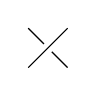
\begin{tikzpicture}[scale = .25, rotate = 90, baseline=-2pt]
    \draw (-1,-1) -- (-0.2,-0.2);
    \draw (0.2,0.2) -- (1,1);
    \draw (-1,1) -- (1,-1);
    \end{tikzpicture}
    
    
    & \stackanchor{++}{++} & \stackanchor{+-}{-+} & \stackanchor{-+}{+-} & \stackanchor{-+}{-+} & \stackanchor{--}{--} \\
    \midrule
    $R(s_0)$ & $x^\frac14 y^\frac14 q^\frac14$ & $x^\frac14 y^{-\frac14}q^{-\frac14}$ & $x^{-\frac14}y^{\frac14}q^{-\frac14}$ & $y^{\frac12}q^\frac14$ & $x^{-\frac14}y^{-\frac14}q^{\frac14}$\\
    \end{tabular}
    \caption{Minimal $x,y$-exponents of $R$ evaluated at the state $s_0$, in terms of the value of $\id$ at a crossing $c$.} 
    \label{tab:xq-pos-contributions}
\end{table}

\begin{table}
    \centering
    \begin{tabular}{c|*{6}{c}}

    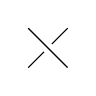
\begin{tikzpicture}[scale = .25, baseline=-2pt]
    \draw (-1,-1) -- (-0.2,-0.2);
    \draw (0.2,0.2) -- (1,1);
    \draw (-1,1) -- (1,-1);
    \end{tikzpicture}
    
    
    & \stackanchor{--}{--} & \stackanchor{+-}{-+} & \stackanchor{-+}{+-} & \stackanchor{+-}{+-} & \stackanchor{++}{++} \\
    \midrule
    $R^{-1}(s_0)$ & $x^\frac14 y^\frac14 q^{-\frac14}$ & $x^{-\frac14} y^{\frac14} q^{\frac14}$ & $x^{\frac14}y^{-\frac14}q^{\frac14}$ & $x^{\frac12}q^{-\frac14}$ & $x^{-\frac14}y^{-\frac14}q^{-\frac14}$\\
    \end{tabular}
    \caption{Minimal $x,y$-exponents of $R^{-1}$ evaluated at the state $s_0$, in terms of the value of $\id$ at a crossing $c$.} 
    \label{tab:xq-neg-contributions}
\end{table}

Denote by $\mathfrak{i}(L)$ the index of a link $L$, defined as
\begin{equation}
    \mathfrak{i}(L) = \frac{|L|-\chi(L)}{2}
\end{equation}
where $\chi(L)$ is the minimal Euler characteristic of all Seifert surfaces bounded by $L$. Since $\chi(L)=1-2g(L)$, we have that
\begin{equation}
    \mathfrak{i}(K)=g(K)
\end{equation}
for any knot $K$.

\begin{proposition} Let $L$ be a homogeneous braid link. Let $\bd\in B_n$ be a homogeneous braid representative for $L$. Then,
\begin{equation}
    \deg_x F_L(x,q)=\mathfrak{i}(L)-\frac12.
\end{equation}
\end{proposition}

\begin{proof}
    Let $N$ denote the number of crossings of $\bd$. From \cref{tab:xq-pos-contributions,tab:xq-neg-contributions} and the formula computing $F_L$ we get that each crossing contributes $1/2$ and each strand contributes $-1/2$ (after normalization). Then,
    \begin{equation}
        \deg_x F_L(x,q) = \frac{N}{2}- \frac{n}{2}.
    \end{equation}
    Let $H^{\pm}$ denote the positive/negative Hopf bands. They are bounded by twisted annuli, therefore $g(H^{\pm})=0$ and $\mathfrak{i}(H^{\pm})=\frac12$. Let $N_{\pm}$ denote the number of positive/negative crossings of $\bd$ and $k_{\pm}$ the number of positive/negative generators. $\bd$ can be obtained from plumbing $N_{+}-k_+$ positive bands and $N_{-}-k_-$ negative bands. The index is multiplicative under plumbing. Therefore, the index of $L$ is
    \begin{equation}
        \mathfrak{i}(L)= \left(N_{+}-k_+\right)\mathfrak{i}(H^+)+\left(N_{-}-k_-\right)\mathfrak{i}(H^-) = \frac{1}{2}\left(N - (n-1)\right).
    \end{equation}
\end{proof}


\begin{proposition} Let $L$ be a homogeneous braid link. Let $\bd$ be a braid representative for $L$ in $\{\sigma_1^{\varepsilon_1},\dots,\sigma_{n-1}^{\varepsilon_{n-1}}\}$. Then,
\begin{equation}
    \ell(L)= \frac{w(\bd)}{4}-\frac12 \sum_{i=1}^{n-1}\varepsilon_i
\end{equation}
\alert{makes sense? For that I also need to study x powers. For h.b.k. it does}
\end{proposition}

\begin{proof} Each crossing contributes $q^{\frac{\sgn(c)}{4}}$ and each closed strand contributes $q^{-\frac{\varepsilon_i}{2}}$.    
\end{proof}

% Q: has symmetry in x and y have anything to do with lk =0?

\notice{Might be worth it to modify the R matrices so we get the Hopf instead of Hopf shifted by writhe. Similarly so that we get ADO back.}

\begin{remark} For a homogeneous braid link $L$ with braid representative $\bd$, $\ell(L)=\mathfrak{i}(L)-\lambda(L)-\frac{w(\bd)}{4}$.
\end{remark}

\notice{Behaviour of Hopf invariant under partial surgery? If we modify the R matrices by the $1/4$, we can use it to find the overall $q$-exponent in the surgery formula!} \alert{Notice that it changes the limits...}

\subsection{Torus links}

From \cite{Park20} we deduce the closed formula
\begin{equation}
    F_{T_{2,2n}}(x,y,q) \factoreq \sum_{m\in\Z} \sgn^+{(m)} q^{n m^2 + m(n-1)} \left(x y\right)^{\sgn^+{(m)}\frac{2 n m+n-1}{2}}
\end{equation}
where $\sgn^+{(0)}=1$. In particular,
\begin{equation}
    F_{T_{2,2n}}(1,1,q) \factoreq \sum_{m\in\Z} \sgn^+{(m)} q^{n m^2 + m(n-1)}= h_{2n}(q).
\end{equation}

Note that $F_{T_{2,4}}(1,1,q)=h_4$ agrees with the tail of $T(2,4)$ (\href{https://arxiv.org/pdf/1106.3948}{Theorem 3.9}). \alert{Check with the non-fibered one.}

(Compare with \href{https://msp.org/agt/2024/24-1/agt-v24-n1-p05-p.pdf}{Table 1} and the formula for $\lambda$ above. Compare for T(3,3) as well)

Note that we have the derivative of the $q$-exponent w.r.t. $m$ divided by $1/2$ times $\sgn^+{(m)}$ in the $x y$ exponent!

\href{https://link.springer.com/book/10.1007/978-3-0348-9227-8}{On the genus depending on orientation of the link components (Example 4.1.4).}

\href{https://stoimenov.net/stoimeno/homepage/papers/quasi2_subl.pdf}{On (2,n) torus links and they are sublinks of index 3 SQP}.

\begin{equation}
    F_{T_{2,4}}(x,y,q) \factoreq \sum_{m\geq 1} (-1)^{m}q^{-\frac{m(m-1)}{2}}y^m x^{m}
\end{equation}
\alert{Partial orientation reversal:}
\begin{equation}
    F^{(1)}_{T_{2,4}^*}(x,y,q) \factoreq \sum_{m\geq 1} (-1)^{m+1}q^{-\frac{m(m-1)}{2}}y^m x^{-m+1}
\end{equation}
\begin{equation}
    F^{(2)}_{T_{2,4}^*}(x,y,q) \factoreq \sum_{m\geq 1} (-1)^{m+1}q^{-\frac{m(m-1)}{2}}y^{-m+1} x^{m}
\end{equation}
and 
\begin{equation}
    F_{\overline{T_{2,4}^*}}(x,x,q) \factoreq \left(\sum_{m\geq 1} (-1)^{m+1}q^{\frac{m(m-1)}{2}}\right) x = h_4(q) x
\end{equation}
which agrees with the stability series of $\overline{T_{2,4}^*}$. \notice{Fix overall term!}

\subsection{Slopes for links}

\begin{example}
For the link $\mathrm{L}7a_1\{0\}$ we have
\begin{equation}
    \delta_{n,m}=\begin{cases}
        -\frac{n-2}{2}m-\frac{n^2}{8}-\frac{n}{4}+1 \quad &n\equiv 0\,(2) \\
        -\frac{n-1}{2}m-\frac{n^2}{8}+\frac18 \quad &n\equiv 1\,(2)
    \end{cases}
\end{equation}
We find that the $n^2$ coefficient is $-1/8$, the $n\cdot m$ is $-1/2$ and the $m^2$ is $0$. \notice{So might be the slope $(-8,0)$?}

Its surgeries ($\pm 1$) are $6_2$ and $6_3$, whose $F_K$ slopes are $-4,8$ and $-6,6$ (I need to find the correct orientation). \notice{check relation (when lk=0).}
\end{example}

\begin{example}
$\mathrm{L}8a5\{0\}$ has $\delta_{n,m}=-(n-1)m$ and $lk=-2$. It's $+1/r$ surgeries is the family $(6_2,8_9,10_9,\cdots)$ which all have the same min. degree quasipolynomial and the same min. slope $-8$. % not two-bridge. Difference of quasipolynomials after doing surgery vs. whitehead? (since almost the same slopes)
\end{example}

\subsubsection{2-bridge links}

Compare with \href{https://arxiv.org/pdf/math/0505442}{this}.

\begin{example} For the Whitehead link $\mathrm{L}5a_1$ ($5_1^2$) we have
\begin{equation}
    \delta_{n,m}=-n m
\end{equation}
\notice{Is this the boundary slope (0,0)?}
\end{example}

\begin{example} $\mathrm{L}7a_5\{1\}$ ($7_2^2$) is the two-bridge link $5/18$ and we have
\begin{equation}
    \delta_{n,m}=-(n - 1) m + \frac12 n(n-1) = \frac{n^2}{2}-n m+\text{(linear terms)}
\end{equation}
and it may be associated to the boundary slope $(1+2s,1-2s)$ at $s=1/2$ i.e. $(2,0)$.
\end{example}

\subsection{Surgery families}

\notice{F.ex.: family L8a5{0} and $(6_2,8_9,10_9...)$ and stabilization of the Fk's. Is the result a power series in $q$ with coefficients rational functions in $x$?}

\section{Multivariable $\rho_1$}

\subsection{Formula}

Let $M$ be as in Section [...]. Assume $\Delta_L(\mathbf{x})\neq 0$ (equivalently, $M$ is not a singular matrix). Let
\begin{equation}
    g_{i,j}(\mathbf{x})= \frac{1-x_{\phi(j)}}{1-x_{\phi(i)}}M^{-1}_{i,j}.
\end{equation}
For a crossing $c$, let
\begin{equation}
    R_1(c)=[...]
\end{equation}
Then, we define
\begin{equation}
    \rho_1(x_1,\dots,x_n)=\rho_1(\mathbf{x})=\Delta_L(\mathbf{x})^2\left(\sum_{c} R_1(c)-[...]\right).
\end{equation}

\begin{example} ($T(2,4)^*$, $T(2,2n)$, ...) [...]
\end{example}

\begin{example} [Whitehead or something complicated]
\end{example}

\begin{example}[The link for which single var alex is zero, but not the multivar]
\end{example}


\subsection{Properties}

% [Lemmas? Similar proofs as with the one-variable case?]

\begin{proposition} 
For a crossing of sign $s$, we have
\begin{equation}
    g_{i,\beta}=\delta_{i,\beta}+x_{\phi(j)}^sg_{i^+,\beta}+(1-x_{\phi(j)}^s)g_{j^+,\beta}, \hspace{1em} g_{j,\beta}=\delta_{j,\beta}+g_{j^+,\beta}, \hspace{1em} g_{2n+1,\beta}=\delta_{2n+1,\beta}
\end{equation}
and
\begin{equation}
    g_{\alpha,i}=x_{\phi(j)}^{-s}\left(g_{\alpha,i^+}-\delta_{\alpha,i^+}\right), \hspace{1em} g_{\alpha,j}=g_{\alpha,j^+}-g_{\alpha,i}(1-x_{\phi(j)}^s)-\delta_{\alpha,j^+}, \hspace{1em} g_{\alpha,1}=\delta_{\alpha,1}.
\end{equation}
\end{proposition}

\begin{remark} For the multivariable case, in the normalization we have chosen, we ``lose'' the interpretation in terms of ``traffic counters''. This interpretation is recovered when we set all variables to be the same. However, in this convention we are able to prove the invariance under Reidemeister moves.
\end{remark}

\begin{proof} For a positive crossing, expanding $(MM^{-1})_{i,\beta}=\delta_{i,\beta}$ gives:
\begin{equation}
    (1-x_{\phi(\beta)})\delta_{i,\beta}=(1-x_{\phi(i)})g_{i,\beta}-(1-x_{\phi(i)})x_{\phi(j)}g_{i^+,\beta}-(1-x_{\phi(j)})(1-x_{\phi(i)})g_{j^+,\beta}
\end{equation}
Therefore, for a positive crossing:
\begin{equation}
    g_{i,\beta}=\delta_{i,\beta}+x_{\phi(j)}g_{i^+,\beta}+(1-x_{\phi(j)})g_{j^+,\beta}
\end{equation}
For a negative crossing we get:
\begin{equation}
    g_{i,\beta}=\delta_{i,\beta}+x_{\phi(j)}^{-1}g_{i^+,\beta}+(1-x_{\phi(j)}^{-1})g_{j^+,\beta}
\end{equation}
For any crossing:
\begin{equation}
    g_{j,\beta}=\delta_{j,\beta}+g_{j^+,\beta}
\end{equation}
and
\begin{equation}
    g_{2n+1,\beta}=\delta_{2n+1,\beta}
\end{equation}
Now, expanding $(M^{-1}M)_{\beta,i}=\delta_{\beta,i}$ gives:
\begin{equation}
    g_{\alpha,i}=x_{\phi(j)}^{-s}\left(g_{\alpha,i^+}-\delta_{\alpha,i^+}\right)
\end{equation}
and
\begin{equation}
    g_{\alpha,j}=g_{\alpha,j^+}-g_{\alpha,i}(1-x_{\phi(j)}^s)-\delta_{\alpha,j^+}
\end{equation}
and
\begin{equation}
    g_{\alpha,1}=\delta_{\alpha,1}
\end{equation} 
\end{proof}

\section{New $F_K$'s for knots}

\notice{Explanation of the method in depth: use surgery to get FK up to overall factor, then use MMR and Alexander to determine the overall factor, whenever the limits are convergent.}

\begin{table}[h!]
    \centering
    \begin{tabular}{|c|c|c|c|}
        \hline
        Knot & $\lc \Delta_K$ & $g(K)$ & Link(s) \\
        \hline
        $6_1$ & $2$ & $1$ & $\mathrm{L}5a_{1},\mathrm{L}7a_{5},\mathrm{L}10n_{25}$ \\
        $8_1$ & $3$ & $1$ & $\mathrm{L}5a_{1}$ \\
        $8_4$ & $2$ & $2$ & $\mathrm{L}7a_{3},\mathrm{L}9a_{24}$ \\
        $8_6$ & $2$ & $2$ & $\mathrm{L}7a_{1},\mathrm{L}9a_{22}$ \\
        $8_8$ & $2$ & $2$ & $\mathrm{L}7a_{1},\mathrm{L}9a_{21}$ \\
        $8_{11}$ & $2$ & $2$ & $\mathrm{L}8a_{2},\mathrm{L}10a_{25}$ \\
        $8_{13}$ & $2$ & $2$ & $\mathrm{L}8a_{4},\mathrm{L}10a_{68}$ \\
        $8_{14}$ & $2$ & $2$ & $\mathrm{L}10a_{11}$ \\
        $9_{12}$ & $2$ & $2$ & $\mathrm{L}8a_{4}$ \\
        $9_{14}$ & $2$ & $2$ & $\mathrm{L}8a_{2},\mathrm{L}10a_{57}$ \\
        $9_{15}$ & $2$ & $2$ & $\mathrm{L}8a_{1}$ \\
        $9_{19}$ & $2$ & $2$ & $\mathrm{L}8a_{1},\mathrm{L}10a_{55}$ \\
        \hline
    \end{tabular}
    \caption{Non-fibered, non-strongly quasipositive knots of at most 9 crossings that can be obtained from partial surgery on a 2-component, homogenoeus braid link. \alert{To do: verify all using is\_isometric\_to.} \notice{Write the whole surgery presentation}}
    \label{tab:knots-and-partial-surgeries}
\end{table}

\begin{table}[h!]
    \centering
    \begin{tabular}{|c|c|c|c|c|}
        \hline
        Knot & $\lc \Delta_K$ & $g(K)$ & $|\sigma|$ & Link(s) \\
        \hline
        $7_3$ & $2$ & $2$ & $4$ & $\left(\mathrm{L}7a_{3}\{0\},+1/2\right)$ \\
        \hline
    \end{tabular}
    \caption{Non-fibered, strongly quasipositive knots of at most 9 crossings that can be obtained from partial surgery on a 2-component, homogenoeus braid link. \alert{To do: verify all using is\_isometric\_to.}}
    \label{tab:knots-and-partial-surgeries}
\end{table}

\begin{table}[]
    \centering
    \begin{tabular}{|c|c|}
        \hline
        Knots & Surgery on: \\
        \hline
        $6_1,8_1,10_1,\cdots$ &  \\
        \hline
        $6_2,8_4,10_4\cdots$ & \\
        $7_3,9_4\cdots$ & \\
        $6_2,8_6,\cdots$ & \\
        $6_3,8_8,10_{34},\cdots$ & \\
        \hline
        $6_2,8_{11},10_7,\cdots$ & $S^3_{+1/r}(\mathrm{L}8a_2\{0\})$\\
        $7_7,9_{14},11a_{195},\cdots$ & $S^3_{-1/r}(\mathrm{L}8a_2\{0\})$ \\
        \hline
    \end{tabular}
    \caption{Families of non-fibered knots that come from partial surgery on the same 2-component, homogeneous braid link.}
    \label{tab:placeholder}
\end{table}

\subsection{The double twist family $K_{n,1}$}

As a warm up, let us review some facts about the $F_K$ invariant of the double twist family $K_{n,1}$.

\subsection{The double twist family $K_{n,-1}$}
We can compute the family of double twist knots $K_{n,-1}$ for $n\geq 2$ by performing different surgeries on the Whitehead link, $\mathrm{L}5a_1$ in \cref{tab:knots-and-partial-surgeries}. Concretely,
\begin{equation} % Choose a better notation. Make the cusp explicit
    S^3_{-\frac1n}(\mathrm{L}5a_1)\cong K_{n,-1}
\end{equation}
for $n\geq 2$. The first examples of this family are $4_1$ (fibered), $6_1, 8_1, 10_1\dots$ (non-fibered), in Rolfsen's notation. % $(2n+2)_1$ in Rolfsen notation % Fix the difference between n\geq 1 and n\geq 2

From \cite{RevisitingMMR}, we find the closed expression for the Habiro coefficients
\begin{equation}\label{eq:Habiro-coeffs-twist}
    a^{K_{n,-1}}_{k_1}(q)=\sum_{k_2\cdots k_n\geq 0} \prod_{j=1}^{n-1}\qbinom{k_j}{k_{j+1}} q^{\sum_{j=2}^{n} k_j(k_j+1)}
\end{equation} % 6_1 has k_2, 8_1 k_2...k_3, etc.
for $n\geq 2$, and $a^{4_1}_{k_1}(q) = 1$ for $n=1$. % here I use qbinom as ration of qpochs

\notice{Even if I prove all of this, it would all be modulo the Whitehead state sum giving what we want}

We find that the $F_K$ candidates we obtain by doing partial surgery on the Whitehead link are precisely
\begin{equation}
    F_{K_{n,-1}}(x,q)\factoreq \sum_{j=0}^\infty \sum_{k_1=0}^j \qbinom{j+k_1}{2j}_q a^{{K_{n,-1}}}_{-k_1-1}(q) x^j
\end{equation} % here []_q is [] in inverted Habiro paper, and viceversa
\alert{prove? qZeil?} where we are using
\begin{equation}
    \qbinom{-k_1}{k_2}=\frac{(q^{-k_1},q^{-1})_{k_2}}{(q)_{k_2}}=(-1)^{k_2}q^{-k_1k_2-\frac{k_2(k_2-1)}{2}}\frac{(q^{k_1},q)_{k_2}}{(q)_{k_2}}
\end{equation}
when evaluating \eqref{eq:Habiro-coeffs-twist} at $-k_1$, with $k_1\geq 0$. Note that $d_{K_{n,-1}}=1=g(K_{n,-1})$ for all $n\geq 1$.

The first coefficient $f_0^{K_{-n,1}}= a_{-1}^{K_{-n,1}}$ is
\begin{equation}
    % a_{-1}^{K_{n,-1}}(q)= \sum_{k_2\dots k_n\geq 0} \frac{(q^{-1})_{k_2}}{(q)_{k_2}} \prod_{j=2}^{n-1} \qbinom{k_j}{k_{j+1}} q^{\sum_{j=2}^{n} k_j(k_j+1)}
    a_{-1}^{K_{n,-1}}(q)= \sum_{k_2\dots k_n\geq 0} (-1)^{k_2} q^{\frac{k_2(k_2+1)}{2}}\prod_{j=2}^{n-1} \qbinom{k_j}{k_{j+1}} q^{\sum_{j=3}^{n} k_j(k_j+1)},
\end{equation}
where we understand the product to be $1$ for $n=2$. In this case, i.e. for the knot $K_{2,-1}=6_1$,
\begin{equation}
    a_{-1}^{6_1}(q) = \sum_{k_2\geq 0} (-1)^{k_2} q^{\frac{k_2(k_2+1)}{2}} = \psi_2(q).
\end{equation}
In fact, $a_{-1}^{K_{n,-1}}$ is equal to false theta $\psi_{n}$ for all values of $n\geq 2$. \alert{qZeil?} We can immediately deduce that
\begin{equation}
    \lim_{q\nearrow 1} f_0^{K_{n,-1}}(q)=\frac{1}{n}=\frac{1}{\lc \Delta_{K_{n,-1}}(x)}.
\end{equation}

The second coefficient $f_1^{K_{-n,1}}= a_{-1}^{K_{-n,1}}+a_{-2}^{K_{-n,1}}$ can be computed from
\begin{equation}
    % a_{-1}^{K_{n,-1}}(q)= \sum_{k_2\dots k_n\geq 0} \frac{(q^{-1})_{k_2}}{(q)_{k_2}} \prod_{j=2}^{n-1} \qbinom{k_j}{k_{j+1}} q^{\sum_{j=2}^{n} k_j(k_j+1)}
    a_{-2}^{K_{n,-1}}(q)= \sum_{k_2\dots k_n\geq 0} (-1)^{k_2} q^{\frac{k_2(k_2-1)}{2}}\frac{1-q^{k_2+1}}{1-q}\prod_{j=2}^{n-1} \qbinom{k_j}{k_{j+1}} q^{\sum_{j=3}^{n} k_j(k_j+1)}.
\end{equation}
We separate $(1-q)a_{-2}^{K_{n,-1}}(q)$ in two terms:
\begin{equation}
\begin{split}
    &\sum_{k_2\dots k_n\geq 0} (-1)^{k_2} q^{\frac{k_2(k_2-1)}{2}}\prod_{j=2}^{n-1} \qbinom{k_j}{k_{j+1}} q^{\sum_{j=3}^{n} k_j(k_j+1)} \quad \text{and}\\
    &-q\sum_{k_2\dots k_n\geq 0} (-1)^{k_2} q^{\frac{k_2(k_2+1)}{2}}\prod_{j=2}^{n-1} \qbinom{k_j}{k_{j+1}} q^{\sum_{j=3}^{n} k_j(k_j+1)}
\end{split}
\end{equation}
The latter series is just $-q\cdot a_{-1}^{K_{n,-1}}(q) = -q\cdot \psi_n(q)$. The former can be written as (experimentally, using Mathematica)
\begin{equation}
\begin{split}
    A_n(q)&=\sum_{j\in \Z} \sgn(j)\left(q^{n j^2-(n-1)j}+q^{n j^2+(n-2)j}\right) = 1-\psi_n(q)+\sum_{j\in \Z} \sgn(j)q^{n j^2+(n-2)j} \\ &=1-\psi_n(q)+B_n(q)
\end{split}
\end{equation}
where $\sgn(0)=0$. Therefore, we can write $f_1^{K_{n,-1}}(q)$ as
\begin{equation}
\begin{split}
    f_1^{K_{n,-1}}(q) &= \frac{1-2q}{1-q}\psi_n(q)+\frac{1}{1-q}A_n(q) \\& =\frac{2q}{1-q}\psi_n(q)+\frac{1}{1-q}\left(B_n(q)+1\right)
\end{split}
\end{equation}
Note $A_2(q)=1-\psi_2(q)$ and $B_n(q)+1$ is the same formula as $B_n$ but changing the sign convention to give $\sgn^+(0)=1$.

\notice{If $n$ is even, $B_n(q)=\psi_{n/2}(q^2)-1=h_n(q^2)-1$. If $n$ is odd, the same thing holds in terms of the $q$-exponents but not $q$-coefficients ($\pm1$). We can modify the definition of $h_n(q)$ to introduce an extra variable $z$ that will allow us to modify the coefficients.} 

As we have mentioned, surgery formulas do not determine the overall $q$-exponent of the resulting $F_K$. However, using the connection to the Melvin-Morton-Rozansky expansion, we can find it by computing the limit at $q=1$ of the first coefficient $f_0(q)$ and its first $q$-derivative.

\begin{example}\label{ex:FK-6_1} For the first knot in the family $6_1$, we obtain
\begin{equation}\label{eq:6_1-FK-coeffs}
\begin{split}
    f_0^{6_1}(q) &\factoreq \psi_2(q)= 1 - q + q^3 - q^6 + q^{10} - q^{15} +\cdots \\
    f_1^{6_1}(q) &\factoreq 1 - q + q^2 + q^3 - q^4 - q^5 - q^6 + q^7 + q^8 + q^9 + q^{10} - q^{11} - q^{12} + \cdots \\
    f_2^{6_1}(q) &\factoreq 1 + q^2 + q^3 - 2 q^4 - 2 q^5 + 2 q^7 + 3 q^8 + q^9 - 3 q^{11} - 3 q^{12} - 2 q^{13} - q^{14} + \cdots
\end{split}
\end{equation}
and $d_{6_1}=1$. To determine the overall $q$-exponent and sign, we look at the (normalized)\footnote{We have added a normalization factor $(1-x^{-1})$.} Melvin-Morton-Rozansky expansion in $h:=1+q$ of $6_1$:
\begin{equation}
   \left(\frac12- \frac{h}{8}+O(h^2)\right) + \left(\frac34 - \frac{h}{16}+O(h^2)\right) x + \cdots
\end{equation}
Given that $\lim_{q\nearrow 1}\psi_2(q)=1/2$, we take the overall sign of $F_{6_1}(x,q)$ to be $+$. For the overall $q$-exponent, we can use the information in the first-order term. We impose
\begin{equation}
    \lim_{q\nearrow 1} \frac{df_0(q)}{dq} = \lim_{q\nearrow 1} \frac{d\left(q^{\ell(6_1)} \psi_2(q)\right)}{dq}=-\frac18.
\end{equation}
Using $\lim_{q\nearrow1}\frac{d\psi_2}{dq}=-1/8$ \alert{cite}, we get $\ell(6_1)=0$. % This is modulo proving that f_0 is the false theta, which we need to do using qZeil

We find the closed formula
\begin{equation}
    f_1^{6_1}(q) \factoreq 1 + \frac{1}{1-q}\sum_{n\geq 1}{q^{2 n^2 + 3n + 2} \left(- q^{- 2 n-1} + 2 - q^{2 n+2}\right)}. % Compare with Sun's for 5_2
\end{equation} % Do these have any value, if we write them above as well? % Notice how f_0 appears inside of f_1, it's very interesting
% Notice that we can rewrite $f_1(q)$ as 
% \begin{equation}
%     [rewrite.in.terms.of.theta.functions]
% \end{equation}
% Using the asymptotics of the well-known theta functions \cite{Theta}
% \begin{equation}
%     [asymptotics]
% \end{equation}
\notice{Can I write it closer to the formula for $f_1$ of $5_2$?} and we check that \alert{expand}
\begin{equation}
    \lim_{q\nearrow 1} f_1(q) = 1-\frac14 =  \frac{3}{4}.
\end{equation}

Note that $\delta_{-j-1}^H = j(j+1)$ (inverted Habiro slopes) \alert{prove} and therefore
\begin{equation}
    f_n(q)=\sum_{j=0}^n \left(q^{-j(n-j)+j(j+1)}+\cdots\right)
\end{equation}
The exponent $j(1+2j-n)$ is minimized for $j=0,\cdots, n$ at $j=Floor(n/4)$ \alert{prove}. Therefore, we get
\begin{equation}
    \delta_n(6_1)=\begin{cases}
        -\frac{n^2}{8}+\frac{n}{4} \quad &n\equiv 0,2\,(4) \\
        -\frac{n^2}{8} + \frac{n}{4} - \frac18 \quad &n\equiv 1\,(4) \\
        -\frac{n^2}{8} + \frac{n}{4} + \frac38 \quad &n\equiv 3\,(4)
    \end{cases}
\end{equation}
Therefore, it picks out the slope $8$.

% Can we do this for the rest of the family?

% Note that 5_2 and 6_1 are similar; same with 7_2 and 8_2, etc. Also all knots also coincide in one of their boundary slope, 4. Find the slope!
\end{example}


A similar study on the other $K_{n,-1}$ twist knots gives $\ell(K_{n,-1})=0$ for all $n\geq 1$. This is consistent with the expectation coming from \cite[Section 7]{L-inv}. % Can we prove using BN code what [...] is for all Kn,-1?
% Add that 8_1 picks slope 12, and what the expectation would be for the rest of the family. We might be able to prove.
The family $K_{k,-1}$ has as slopes $-4,0,4k$ and their min degs are
\begin{equation}
    \delta_n(K_{k,-1})=\min_{0\leq j\leq n}{(k-1)j(j+1)-j(n-j)} = \min_{0\leq j\leq n}{kj^2-n j+(k-1)j}.
\end{equation}
where $(k-1)j(j+1)$ is the minimum degree of the inverted Habiro coefficient $a_{-1-j}^{K_{k,-1}}(q)$. For $6_1$, minimum was attained at $j=Floor(n/4)$. For $8_1$ we want the leading term to be $-n^2/12$ and the leading term is $3j^2-n j$; if $j=n/a$ we must have $3/a^2-1/a=-1/12\Rightarrow a^2-12a+36=(a-6)^2=0\Rightarrow a=6$. The leading term in general is $k j^2$ and if $j=n/a$ we want $k/a^2-1/a=-1/(4k)\Rightarrow a^2-4k a+4k^2=(a-2k)^2=0 \Rightarrow a=2k$. We just need to prove that $j=Floor(n/(2k))$ minimizes that quantity, and we have a prove that the $F_K$ slope is $4k$ for the whole family.

Notice that if $j=\frac{n+b}{2k}$, we get
\begin{equation}
    -\frac{n^2}{4k}+\frac{k-1}{2k}n + \frac{(k-1)}{2k}b.
\end{equation}
From which we prove that the first-order coefficient is also an integer for all $n$, and the only term that is periodic is the constant. \notice{Can we find the constant theoretically?}

\begin{remark} We notice that $F_{6_1}(x,q)$ is very similar to $F_{5_2}(x,q)$ (see \cite[Eq. 31]{Park20})\footnote{We write $5_2$ what is $m(5_2)$ in the convention of \cite{Park20}.}. We find the relations:
\begin{equation}\label{eq:FK-6_1-5_2}
\begin{split}
    f_0^{6_1}(q) &= -q f_0^{5_2}(q) \\
    f_1^{6_1}(q) &= 1+q^2f_1^{5_2}(q)\\
\end{split}
\end{equation}
It is known that $f_0^{5_2}(q)$ and $f_1^{5_2}(q)$ are related to each other (deduced from a relation between the corresponding inverted Habiro coefficients found in \cite{Park21})\footnote{We thank J. Sbovoda for the suggestion.} \alert{Can we prove it?}
\begin{equation}
    q\left((1-q)f_1^{5_2}(q)-2f_0^{5_2}(q)\right) = 1.
\end{equation}
Using \eqref{eq:FK-6_1-5_2}, we obtain an analogous relation between the first two coefficients of $F_{6_1}(x,q)$.

The similarities continue when we compare $F_{8_1}(x,q)$ to $F_{7_2}(x,q)$. In this case,
\begin{equation}
    f_0^{8_1}(q) = -q f_0^{7_2}(q)
\end{equation}
and
\begin{equation}
\begin{split}
    (1-q)f_1^{8_1}(q)+2qf_0^{8_1}(q) &= q\left((1-q)f_1^{7_2}(q)-2f_0^{7_2}(q)\right) =  1 - \sum_{m\geq 1} (\sgn{m}) q^{m(3m - 1)}
\end{split}
\end{equation}
Therefore, we can write the relation
\begin{equation}
    f_1^{8_1}(q)=q f_1^{7_2}(q) + 2 f_0^{8_1}(q).
\end{equation}
While it is not clear what the structure of the relation between the $K_{n,1}$ and $K_{n,-1}$ families is, it seems like there is a connection for the first examples.

We obtain similar results when comparing $F_{10_1}(x,q)$ to $F_{9_2}(x,q)$, etc. We find that the first two coefficients of both families are related via:
\begin{equation}
\begin{split}
    f_0^{K_{n,-1}}(q)&=-qf_0^{K_{n,1}}(q) \\
    f_1^{K_{n,-1}}(q)&=\alert{...}f_1^{K_{n,1}}(q) \\
\end{split}
\end{equation}

Unlike in the case of the $K_{n,1}$ family, $F_{K_{n,-1}}(x,q)$ does not agree with the stability series of the knot. \notice{Check the rest 81 vs 72 etc.}
\end{remark}

% Make this two sentences coherent with one another

We observed that $4$ is a boundary slope for all knots in both the families $K_{n,-1}$ and $K_{n,1}$. \notice{can we prove for all?}

\begin{remark} In \cite{L-inv} it is asked whether $\min\deg f_0=\min\deg f_1$ for all alternating knots. It is easy to check that, for the family $K_{n,-1}$, we have 
\begin{equation}
    \min\deg f_0^{K_{n,-1}}=\min\deg f_1^{K_{n,-1}}=0.
\end{equation} % Do the actual math!!
\end{remark}

\subsection{Alternating knots}

The fact that the thetas $\psi_n(q)$ appear as the $f_0(q)$ of most examples (with $\lc \Delta_K=n$) allows us to compute the associated $\ell(K)$ theoretically and compare our results with the expectation from \cite[Section 7]{L-inv}.

We compute the examples from \cref{tab:knots-and-partial-surgeries} and write the first three $F_K$ coefficients in \cref{tab:first-FK,tab:second-FK,tab:third-FK}. Surprisingly, there are many series that appear as the $F_K$ coefficients of different knots! This is most common for the first $F_K$ coefficient $f_0$, a bit less common for the second coefficient $f_1$, etc.

We also re-compute some strongly quasipositive examples using the surgery presentation. In particular, we compute:
\begin{equation}
    7_3,9_4,\cdots
\end{equation}
We have verified that the first three $F_K$ coefficients agree with the computation done using the stratified state sum described in \cite{Park20,L-inv} up to \notice{($q$-order)} whenever the stratified sum converges. We have added closed formulas for these series to \cref{tab:second-FK}.

For $7_3$, the stratified sum converges, and agrees with the surgery $F_K$. For $9_4$, the stratified sum does not converge, and this provides another computation. We have checked that it agrees with the stability series for the first 3 terms and first few $q$-terms.

\begin{example} Take the first non-twist knot example in \cref{tab:knots-and-partial-surgeries}, the alternating knot $8_4$. Using the surgery presentation
\begin{equation}
    S^3_{-\frac12}\left(\mathrm{L}7a_3\{0\}\right)\cong 8_4
\end{equation}
we can compute $F_{8_4}(x,q)$ from $F_{\mathrm{L}7a_3\{0\}}(x,y,q)$, which yields
\begin{equation}
\begin{split}
    f_0(q)&\factoreq 1 - q + q^3 - q^6 + q^{10} - q^{15} + \cdots \expeq \psi_2(q) \\
    f_1(q)&\factoreq 1 - q + q^2 + q^3 - q^4 - q^5 - q^6 + q^7 + q^8 + q^9 + q^{10} + \cdots \\
    f_2(q) &\factoreq 1 - q + 2 q^2 - 3 q^4 - q^5 + q^6 + 3 q^7 + 2 q^8 - q^{10} - 4 q^{11} + \cdots
\end{split}
\end{equation}
and $d_{8_4}=2$. % note this is different from its tail

The first two terms coincide with those of the knot $6_1$, whereas they start differing from each other at the third. Notice that their Alexander polynomials are very similar, and therefore its inverse expansions are as well:
\begin{equation}\label{eq:6_1-8_4-alexander-expansion}
    \frac{(1-x^{-1})}{\Delta_{6_1}(x)}=\frac12 + \frac{3 x}{4} + \frac{11 x^2}{8}+\cdots \quad \text{ and } \quad \frac{(1-x^{-1})}{\Delta_{8_4}(x)}=\frac{x}{2} + \frac{3 x^2}{4} + \frac{5 x^3}{8}+\cdots
\end{equation}
Therefore, the third term $f_2(q)$ must be different for both $6_1$ and $8_4$, since we expect their $q=1$ limit to be different. From \eqref{eq:6_1-8_4-alexander-expansion} we also deduce that the overall sign of $F_{8_4}(x,q)$ is $+$. \notice{Q to D: is it understood what I mean?}

To determine the overall $q$-exponent, we look at the (normalized)\footnote{We have added a normalization factor $(1-x^{-1})$.} Melvin-Morton-Rozansky expansion in $h:=1+q$ of $8_4$:
\begin{equation}
   \left(\frac12+ \frac{3h}{8}+O(h^2)\right) x + \left(\frac34 + \frac{11 h}{16}+O(h^2)\right) x^2 + \cdots
\end{equation}
In this case it is important to use the correct orientation of the knot and its corresponding expansion. Otherwise, we would get an incorrect $\ell$ value. This was less important in Example \ref{ex:FK-6_1} since $\ell(6_1)=0$.

Since the first-order term detects the overall $q$-exponent, we must impose
\begin{equation}
    \lim_{q\nearrow 1}\frac{d\left(q^{\ell(8_4)}\psi_2(q)\right)}{dq} = \frac{3}{8},
\end{equation}
from which we deduce that $\ell(8_4)=\frac{|\sigma(8_4)|}{2}=1$. \notice{Make sure to write explicit orientation!}

The same thing happends for $8_1$ and $10_4$ (the first 2 terms are the same, the third is different).
\end{example}

% Change all h_4 for \psi_2

\notice{Q: why do all of these knots have such similar series? What are the properties of a $q$-series for it to be the coefficient of a knot? In particular, for each $f_j$ we get a different possible set of series.}

\notice{What is special about the knots that recover MMR in terms of what link they come from vs. the ones that do not?}

\notice{How to structure all these different series?}

\begin{table}[h!]
    \centering
    \begin{tabular}{|c|c|}
        \hline
        Knots & $|\ell(K)|$ \\
        \hline
        $6_1,8_{1,8,13},9_{14,19}$ & 0 \\
        $8_{4,11},9_{12,15},10_4$ & 1 \\
        \hline
    \end{tabular}
    \caption{Alternating, non-fibered knots and their $\ell$-invariant. We find that $2|\ell(K)|=|\sigma(K)|$ for all the knots in the table.}
    \label{tab:L-invariant}
\end{table}

\begin{table}[h!]
    \centering
    \begin{tabular}{|c|c|c|}
        \hline
        Knots & Series & $f_0(1)$ \\
        \hline
        $6_1, 8_{4,6,8,11,13},9_{12,14,15,19}$ & $\psi_2(q)$ & $1/2$ \\
        $8_1,10_{4,7},11a_{195}$ & $\psi_3(q)$ & $1/3$ \\
        \hline
    \end{tabular}
    \caption{Knots by their first $F_K$ coefficient $f_0^K(q)$, normalized to start at 1. The overall $q$-exponent is recorded in \cref{tab:L-invariant} and the overall sign is given by $-\sgn{\left(\lc \Delta_K\right)}$.}
    \label{tab:first-FK}
\end{table}

\begin{comment}
\begin{table}[h!]
    \centering
    \begin{tabular}{|c|c|c|c|}
        \hline
        Knot & Surg. pres. & $\ell(K)$ & Series \\
        \hline
        $6_1$ & & 0 & $1 - q + q^2 + q^3 - q^4 - q^5 - q^6 + q^7 + q^8 + q^9 + q^{10} + \cdots$ \\
        $8_1$ & & 0 & $1 - q + q^4 + q^5 - q^6 - q^7 - q^8 + q^9 + q^{14} + q^{15} + q^{16} + \cdots$ \\
        $8_4$ & & $1$ & $1 - q + q^2 + q^3 - q^4 - q^5 - q^6 + q^7 + q^8 + q^9 + q^{10} + \cdots$ \\
        $8_8$ & & & $2\psi_2(q)$ \\
        \hline
    \end{tabular}
    \caption{Second $F_K$ coefficient $f_1^K$. We normalize the $F_K$ so that the $f_0$ agrees with \cref{tab:first-FK}.}
    \label{tab:second-FK}
\end{table}
\end{comment}

\begin{table}[h!]
    \centering
    \begin{tabular}{|c|c|c|}
        \hline
        Knots & Series & $f_1(1)$ \\
        \hline
        $5_2, 7_3$ & $\qintTheta_1(q)$ & $1/4$ \\ % I add it since we don't discuss the second onwards in L-invariant paper
        $7_5,9_6,9_9$ & $2\qintTheta_1(q)$ & $1/2$ \\ % s.s. SQP, not surgery, but interesting
        $6_1,8_4$ & $1 -q\qintTheta_1(q)$ & $3/4$ \\ %  = 1 - q + q^2 + q^3 - q^4 - q^5 - q^6 + q^7 + q^8 + q^9 + q^{10} + \cdots
        \alert{$9_{16}$} & $\alert{3\phi_1(q)}$ & $3/4$ \\ % SQP, not surgery & not 2-bridge
        $8_6,8_8$ & $2\psi_2(q)$ & $1$ \\
        $8_{11},8_{13}$ & $3\psi_2(q) - q^2 \phi_3(q)$ & $5/4$ \\
        $\alert{8_{14}}$ & $\alert{4\psi_2(q)-2q^2\phi_3(q)}$ & $3/2$ \\ % ISS, not surgery
        $9_{12},9_{14}$ & $3\psi_2(q) + q^2\phi_3(q)$ & $7/4$ \\
        $9_{15},9_{19}$ & $4\psi_2(q)$ & $2$ \\
        \hline
        $8_1,10_4$ & $\left(1-2\psi_3(q)\right)/(1-q)-q^2(1+q)\bar{\phi}_{3,5}(q^2)$ & $4/9$ \\ % $\left(1-2\psi_3(q) - \sum_{m\in\Z} (\sgn{m}) q^{m(3m - 1)}\right)/(1-q)$
        $10_7$ & $3\psi_3(q) + q^4\left(-\bar{\phi}_{6,14}(q)-\bar{\phi}_{6,20}(q)+q^2(1+q)\bar{\phi}_{3,8}(q^2)\right)$ & $8/9$ \\
        $11a_{195}$ & $3\psi_3(q) - q^4\left(-\bar{\phi}_{6,14}(q)-\bar{\phi}_{6,20}(q)+q^2(1+q)\bar{\phi}_{3,8}(q^2)\right)$ & $10/9$ \\
        \hline
    \end{tabular}
    \caption{Second $F_K$ coefficient $f_1^K$ for alternating, non-fibered knots (up to overall sign and $q$-power).}
    \label{tab:second-FK}
\end{table}

Define $\qintTheta_b(q):=\sum_{n\geq 0}(-1)^nq^{\frac{n(n+b)}{2}}\frac{1-q^{n+1}}{1-q}$. Note you can write $\qintTheta_1$ as a rational function in terms of $\psi_2$.

Define also $\bar{\phi}_{a,b}(q):=\sum_{n\geq 0} q^{\frac{an^2+bn}{2}}\frac{1-q^{n+1}}{1-q}$.

We have
\begin{equation}
    -q^2 (1+q)\bar{\phi}_{3,5}(q^2)=-\frac{1}{1-q}\left(\sum_{m\in\Z} (\sgn{m}) q^{m(3m - 1)}\right)
\end{equation}

\begin{table}[h!]
    \centering
    \begin{tabular}{|c|c|c|}
        \hline
        Knots & Series & $f_2(1)$\\
        \hline
        $6_1$ & (C-poly) & $11/8$ \\
        $8_1$ & (C-poly) & $?$ \\
        $8_4$ & & $5/8$ \\
        $8_6$ & &  $?$ \\
        $8_8$ & $ -1-q+q^2-q^8 \qintTheta_7(q)+4\psi_2(q)$ & $?$ \\ % w/ a -q^0 in front
        $8_{11}$ & & \\
        $9_{14}$ & & \\
        \hline
    \end{tabular}
    \caption{Third $F_K$ coefficient $f_2^K$. We normalize the $F_K$ so that the $f_0$ agrees with \cref{tab:first-FK}.}
    \label{tab:third-FK}
\end{table}

% First non-alternating knot with funky top HFK: 11 crossings! So everything should work for these, and then I should treat the ones with weird HFK etc. separately.


\newpage
\begin{table}[h!]
    \centering
    \begin{tabular}{|c|c|c|}
        \hline
         Knot & $\lc \Delta_K$ & $g(K)$ \\
         \hline
         $10_4$ & 3 & 2 \\
         $10_6$ & 2 & 3 \\
         $10_7$ & 3 & 2 \\
         $10_8$ & 2 & 3 \\
         $10_{10}$ & 3 & 2 \\
         $10_{12}$ & 2 & 3 \\
         $10_{15}$ & 2 & 3 \\
         $10_{19}$ & 3 & 2 \\
         $10_{20}$ & 3 & 2 \\
         $10_{21}$ & 2 & 3 \\
         $10_{22}$ & 2 & 3 \\
         $10_{23}$ & 2 & 3 \\
         $10_{25}$ & 2 & 3 \\
         $10_{26}$ & 2 & 3 \\
         $10_{28}$ & 4 & 2 \\
         $10_{34}$ & 3 & 2 \\
         $10_{50}$ & 2 & 3 \\
         $10_{51}$ & 2 & 3 \\
         $10_{52}$ & 2 & 3 \\
         $10_{54}$ & 2 & 3 \\
         $10_{61}$ & 2 & 3 \\
         $10_{65}$ & 2 & 3 \\
         $10_{72}$ & 2 & 3 \\
         $10_{83}$ & 2 & 3 \\
         $10_{86}$ & 2 & 3 \\
         $10_{135}$ & 3 & 2 \\
         $10_{146}$ & 2 & 2 \\
         $10_{147}$ & 2 & 2 \\
         $10_{162}$ & 3 & 2 \\
         $10_{164}$ & 3 & 2 \\
         \hline
    \end{tabular}
    \caption{Non-fibered, non-strongly quasipositive 10-crossing knots that can be obtained from partial surgery on a 2-component, homogeneous braid link.}
    \label{tab:placeholder}
\end{table}

Look for knots that have the same term in MMR but not the same series!

\notice{Table for knot orientations?}

\notice{Comment about inverted stratified sum and a separate publication.}

\subsection{Non-alternating examples}

The only non-alternating examples up to 10 crossings are: $10_{135,146,147,162,164}$. We compute them as:
\begin{itemize}
    \item $S^3_{+1}(\mathrm{L}10a_{60}\{0\})\cong 10_{135}$
    \item $S^3_{-1}(\mathrm{L}9a_{20}\{0\})\cong 10_{146}$
    \item $S^3_{+1}(\mathrm{L}9a_{31}\{0\})\cong 10_{147}$
    \item $S^3_{+1}(\mathrm{L}10a_{80}\{1\})\cong 10_{162}$
    \item $S^3_{+1}(\mathrm{L}10a_{79}\{1\})\cong 10_{164}$
\end{itemize}

Curiously, they all have linking number $\pm 1$. All of them also satisfy that 
\begin{equation}
    |m-a|=2|\sigma|
\end{equation}
where $(m,a)$ are the Maslov and Alexander grading of top HFK and $\sigma$ is signature. Therefore, we cannot use them to discern whether $\ell$ reads signature or the Maslov grading. What is more, their knot Floer homology is ``alternating-like'' for all of them.
% https://knotinfo.org/results.php?searchmode=advancedsearch&desktopmode=0&mobilemode=0&singleknotprev=&submittype=advancedsearch&searchfield1=alternating&searchoperator1=%3D&searchvalue1=N&searchadjunction1=and&searchfield2=fibered&searchoperator2=%3D&searchvalue2=N&searchadjunction2=and&searchfield3=crossing_number&searchoperator3=%3C&searchvalue3=11&searchadjunction3=and&searchfield4=&searchoperator4=%3D&searchvalue4=&searchadjunction4=and&searchfield5=&searchoperator5=%3D&searchvalue5=&searchadjunction5=and&generalsearchexpr=&name=%3D1&three_genus=%3D1&signature=%3D1&smooth_four_genus=%3D1&hfk_polynomial=%3D1

\begin{example} $10_{146}$. We have $f_0(q)=\psi_2(q)$, $f_1(q)$ decomposes in a similar manner as other series and $\ell(10_{146})=0$.
\end{example}

Interesting examples 11-crossings: 11n34 11n39 11n42 11n45 11n67 11n73 11n79 11n97 11n126 11n138 11n151 11n155. None of them I could find as partial surgeries on homogeneous braid links. i.e. so far all I could find using this procedure are quasi alternating (in the knot Floer sense). However, we are working with low-crossing examples which does not allow to make a strong statement.

\begin{table}[h!]
    \centering
    \begin{tabular}{|c|c|}
        \hline
        Knots & $|\ell(K)|$ \\
        \hline
        $10_{146}$ & 0 \\
        \hline
    \end{tabular}
    \caption{Non-alternating, non-fibered knots and their $\ell$-invariant. We find that $2|\ell(K)|=|\sigma(K)|$ for all the knots in the table.}
    \label{tab:L-invariant-nonalt}
\end{table}

Non-quasi alternating knots that we can find doing partial surgeries on links start at 12 crossings. 

\subsection{Non quasi-alternating}

\begin{example} $12n_{293}$ is also strongly quasipositive, so we can compute using the stratified state sum. We compute it in \cite{L-inv} and we obtained
\begin{equation}
\begin{split}
    f_0(q) &= \Phi_{0}(q)= q^{-2}\sum_{n\geq 0} q^{n^2}
\end{split}
\end{equation}
and $d(12n_{293})=2$. We find the surgery presentation 
\begin{equation}
    S^3_{+1}(\mathrm{L}10a_{89}\{0\})=12n_{293}.
\end{equation}
and it gives
\begin{equation}
    f_0(q) \factoreq q^{-1}\sum_{n\geq 1} q^{n^2} = q^{-1}(-1+\Phi_0(q))
\end{equation}
\end{example}
The surgery $f_1(q)$ is
\begin{equation}
    f_1(q)=\sum_{n\geq 2} q^{n^2} - 2\sum_{n\geq 0} q^{n(n-1)} \frac{1-q^n}{1-q}
\end{equation}

% \notice{Q: are all knots in my list that are non-alternating, SQP?}

% 12n277, 12n546 12n447 12n147 12n565 12n559 12n311 ... appear but are quasi alternating

% 12n457 only one non SQP non quasialternating, non alternating

The knot $12n_{457}$ is non quasi-alternating and non strongly quasipositive. Using the surgery presentation $S^3_{+1}(\mathrm{L}9a_{42}\{0\})\cong 12n_{457}$ we get the same $f_0(q)$ as $12n_{293}$ by surgery. \alert{!}

% Double checks on SQP: https://knotinfo.org/results.php?searchmode=advancedsearch&desktopmode=0&mobilemode=0&singleknotprev=&submittype=advancedsearch&searchfield1=alternating&searchoperator1=%3D&searchvalue1=N&searchadjunction1=and&searchfield2=fibered&searchoperator2=%3D&searchvalue2=N&searchadjunction2=and&searchfield3=crossing_number&searchoperator3=%3C&searchvalue3=13&searchadjunction3=and&searchfield4=strongly_quasipositive&searchoperator4=%3D&searchvalue4=Y&searchadjunction4=and&searchfield5=&searchoperator5=%3D&searchvalue5=&searchadjunction5=and&generalsearchexpr=&name=%3D1&three_genus=%3D1&signature=%3D1&smooth_four_genus=%3D1&hfk_polynomial=%3D1

% Taking out SQP: https://knotinfo.org/results.php?searchmode=advancedsearch&desktopmode=0&mobilemode=0&singleknotprev=&submittype=advancedsearch&searchfield1=alternating&searchoperator1=%3D&searchvalue1=N&searchadjunction1=and&searchfield2=fibered&searchoperator2=%3D&searchvalue2=N&searchadjunction2=and&searchfield3=crossing_number&searchoperator3=%3C&searchvalue3=13&searchadjunction3=and&searchfield4=strongly_quasipositive&searchoperator4=%3D&searchvalue4=N&searchadjunction4=and&searchfield5=&searchoperator5=%3D&searchvalue5=&searchadjunction5=and&generalsearchexpr=&name=%3D1&three_genus=%3D1&signature=%3D1&smooth_four_genus=%3D1&hfk_polynomial=%3D1

\begin{example} The knot $13n_{3663}$ can be obtained using the surgery presentation
\begin{equation}
    S^3_{-1}(\mathrm{L}?)\cong 13n_{3663}.
\end{equation}
This is a non-quasialternating knot. It is unknown whether it is strongly quasipositive. The Alexander polynomial is $\Delta_{13n_{3663}}(x)=x^{-1}-1+x$ and its MMR up to first order is:
\begin{equation}
    \left(1-3 h +O(h^2)\right) x+\left(1-7 h+O(h^2)\right) x^2+\left(-h+O(h^2)\right) x^3+O(x^4)
\end{equation}
Its knot Floer polynomial is:
\begin{equation}
    (m^{-1} + 2)a^{-1}+ (3 + 4m)+ (m + 2m^2)a
\end{equation}
and
\begin{equation}
    f_0(q)=1 + q^3 + q^8 - q^9 + q^{15} - q^{16} - q^{17} + q^{24} - q^{25} - q^{26} + q^{35} - q^{36} - q^{37} + q^{40} + \cdots
\end{equation}

\end{example}

\subsection{Slopes after using partial surgery}

\notice{I need to read \href{https://arxiv.org/pdf/math/0505442}{[this]} and similar. $4_1^2$ is probably $T(2,4)^+$ and we pick the $(-2,-2)$, but I don't know how to relate that to $\delta_{n,m}$ yet.}

Let $L$ be a 2-component link with linking number $lk\geq 0$. Then,
\begin{equation}
\begin{split}
    F_{S^3_{-1}(L)}(x,q)&=\mathcal{L}\left(x^\frac12 \sum_{n,m=0}^\infty \left(q^{\delta_{n,m}^L}+\cdots\right) (y^{m+1}-y^m) x^n \right)
    \\&=x^{\frac12}\sum_{n,m=0}^\infty \left(q^{\delta_{n,m}^L+(m+1)^2}x^{n+lk\cdot (m+1)}-q^{\delta_{n,m}^L+m^2}x^{n+lk\cdot m}+\cdots\right) %  = x^{\frac12}\sum_{k=0}^\infty \left(\sum_{m=0}^\infty q^{\delta^L_{k-lk\cdot m,m}+m^2}+\cdots\right) x^{k}
\end{split}
\end{equation}
Assume $lk=0$. Then,
\begin{equation}
    \delta_k^{S^3_{-1}(L)} = \alert{\min_{0\leq m \leq \infty} \delta_{n,m}+m^2}
\end{equation}

\begin{example} $L=T(2,4)^+$ has (we omit the overall $1/2$)
\begin{equation}
    \delta^{T(2,4)^+}_{n,m} = \begin{cases}
        \frac{m(m+1)}{2} \quad &\text{if }n=m \\
        0 \quad &\text{else}
    \end{cases}
\end{equation}
\notice{How to write as quasipoly?}

Either way, $-1$ surgery gives:
\begin{equation}
    \delta_k = \min_{0\leq m \leq \infty} \delta_{k-2m,m}+m^2
\end{equation}
is attained when $m=0$, which gives $0$. \alert{But this is wrong!}


    
\end{example}

\section{refs}

\href{https://msp.org/agt/2024/24-1/agt-v24-n1-p05-p.pdf}{Alexander detects linking number of 2 component links (page 6).} 
% left off: finding codes to compute link floer homology and reading about it

\href{https://www.its.caltech.edu/~yini/Published/LinkGenus.pdf}{Link genus and link Floer homology}

\href{https://d.lib.msu.edu/etd/52050?__goaway_challenge=header-refresh&__goaway_id=a2e9fb621b09544af78771ab27e5af18&__goaway_referer=https%3A%2F%2Fd.lib.msu.edu%2F}{Computations of link Floer homology and code}

\href{https://arxiv.org/pdf/math/0601618}{Link Floer homology and Thurston norm} (Same statement as Yi Ni but with link Floer)

\href{https://msp.org/agt/2024/24-1/agt-v24-n1-p05-p.pdf}{Link detection and Floer homologies}

\href{https://link.intlpress.com/JDetail/1806601803955335169}{Examples link/knot Floer for links}

\href{https://www.liverpool.ac.uk/~su14/papers/multiburau.pdf}{Multivariable Alexander}

\section{Future ideas}
\begin{itemize}
    \item According to \href{https://www.its.caltech.edu/~yini/Published/LinkGenus.pdf}{Rmk 1.2}, links that have $\Delta_L\equiv 0$ still have non trivial link Floer homology. Can we compute any such 2-component link by doing partial surgery on a 3-component homogenoeus link? (similarly to how we compute the new knots). Or maybe a SQP one!
\end{itemize}

\section*{References}
\printbibliography[heading=none]

\end{document}